\chapter{Υλοποίηση}
\label{chapter:implementation}

Στο κεφάλαιο αυτό θα περιγράψουμε την πειραματική υλοποίηση που πραγματοποιήθηκε στα πλαίσια αυτής της διπλωματικής εργασίας. Πρόκειται για την υλοποίηση Βασικών Υπορουτινών Γραμμικής Άλγεβρας (Basic Linear Algebra Subprograms ή BLAS) Επιπέδου 1 για Ασφαλή Υπολογισμό Δύο Μερών η οποία βασίζεται στη βιβλιοθήκη ABY για την εκτέλεση των πρωταρχικών κρυπτογραφικών και ασφαλούς υπολογισμού διεργασιών. Την βιβλιοθήκη που υλοποιήσαμε ονομάζουμε MPC-BLAS, ωστόσο ένα ίσως καταλληλότερο όνομα θα ήταν το 2PCBLAS. Πρωτού περάσουμε στην ανάλυση της MPC-BLAS βιβλιοθήκης, πρέπει πρώτα να αναλύσουμε ένα λιγότερο κρυπτογραφικό κομμάτι αυτής της εργασίας, τις απλές BLAS βιβλιοθήκες.


\section{Η διεπαφή BLAS}

Η Γραμμική Άλγεβρα αποτελεί πλέον θεμελιώδες μαθηματικό εργαλείο των θετικών επιστήμων, για αυτό και αποτελεί βασικό μάθημα των πρώτων ετών των προπτυχιακών σπουδών σε σχεδόν όλες τις σχολές θετικών επιστημών. Εξετάζοντας μόνο την επιστήμη της πληροφορικής, τη βλέπουμε σε πάρα κλάδους της, όπως τη Μηχανική Μάθηση (π.χ. SVM), στην Ψηφιακή Επεξεργασία Σημάτων (π.χ. FFT), στην Αριθμητική Ανάλυση, στην Κρυπτογραφία (π.χ. Κρυπτογραφία Πλεγμάτων), στα Γραφικά Υπολογιστών (π.χ. Ray Tracers) καθώς και σε πολλούς ακόμα.
Η μαζικότητα αυτή, της χρήσης της γραμμικής άλγεβρας, δημιούργησε από τα πρώτα χρόνια των γλωσσών προγραμματισμού την επιτακτική ανάγκη για την εκτέλεση γρήγορων πράξεων γραμμικής άλγεβρας. Έτσι, από τα χρόνια της γλώσσας Fortran, εγκαθιδρύθηκε από το BLAS Technical Forum ένα πρότυπο \cite{blackford2002updated}, μια διεπαφή συναρτήσεων, την οποία μπορούν να χρησιμοποιούν τα προγράμματα Fortran. Το πρότυπο αυτό πήρε το όνομα \textbf{BLAS (Basic Linear Algebra Subprograms ή BLAS)}. Ο σκοπός της διεπαφής αυτής είναι η υλοποίηση να μπορεί να είναι διαφορετική
από πλατφόρμα σε πλατφόρμα, ώστε να εκμεταλλεύεται τις ιδιομορφίες του υλικού της κάθε πλατφόρμας. Κρατώντας τη διεπαφή σταθερή δε χρειάζεται να αλλάξει ένα πρόγραμμα που τη χρησιμοποιεί. Το μόνο που χρειάζεται, είναι να ξανά μεταγλωττιστεί το πρόγραμμα για τη συγκεκριμένη πλατφόρμα και να συνδεθεί (linked) με τη νέα BLAS υλοποίηση. Μάλιστα στην περίπτωση που η BLAS υλοποίηση υποστηρίζει δυναμική σύνδεση (dynamic linking) μπορεί να μην είναι απαραίτητο να ξαναμεταγλωττιστεί το πρόγραμμα για τη συγκεκριμένη πλατφόρμα. Με την έλευση της γλώσσας C, δημιουργήθηκε αντίστοιχη διεπαφή για τη C αντίστοιχη με αυτή της Fortran. Έχει επικρατήσει να καλούμε τη διεπαφή για τη Fortran ως BLAS ενώ για τη C ως CBLAS.

Γενικότερα, η ύπαρξη τέτοιου είδους διεπαφής δίνει τη δυνατότητα σε κατασκευαστές υλικού, για παράδειγμα επεξεργαστών ή καρτών γραφικών, να δημιουργήσουν BLAS υλοποιήσεις που να εκμεταλλεύονται τα χαρακτηριστικά του κάθε υλικού τους. Έτσι, σήμερα υπάρχουν στη βιβλιογραφία πάρα πολλές υλοποιήσεις της διεπαφής BLAS, ανοιχτού ή κλειστού κώδικα, από ποικίλους συγγραφείς, μεταξύ των οποίων και οι μεγαλύτεροι κατασκευαστές υλικού επεξεργαστών, ακόμα και καρτών γραφικών.

Η διεπαφή BLAS, χωρίζεται σε τρία επίπεδα. Το δεύτερο επίπεδο περιέχει πράξεις μόνο μεταξύ διανυσμάτων ή γενικότερα πράξεις επάνω σε διανύσματα, όπως για παράδειγμα η εύρεση της θέσης του στοιχείου με τη μεγαλύτερη απόλυτη τιμή (πράξη IxAMAX). Το δεύτερο επίπεδο περιέχει μόνο πράξεις μεταξύ πινάκων και διανυσμάτων ενώ το τρίτο επίπεδο περιέχει μόνο πράξεις μεταξύ πινάκων. Στα πλαίσια της εργασίας αυτής θα αναφερθούμε μόνο στις πράξεις του πρώτου επιπέδου οι οποίες φαίνονται συνοπτικά και με αφαιρετικό τρόπο στο Σχήμα \ref{code:blas-level-1}. Ολόκληρη η διεπαφή BLAS βρίσκεται στον παρακάτω \href{https://netlib.org/lapack/explore-html/de/da0/cblas_8h_source.html}{σύνδεσμο}. Οι ονομασίες που χρησιμοποιούνται για τις συναρτήσεις και τις υπορουτίνες είναι στη μορφή xDOT. Το x είναι ένας χαρακτήρας μπαλαντέρ που παίρνει τιμές S, D, C, Z ανάλογα με το αν αναφερόμαστε σε πραγματικούς αριθμούς, μονής ή διπλή ακρίβειας, ή σε μιγαδικούς αριθμούς, μονής ή διπλής ακρίβειας, αντίστοιχα. Για παράδειγμα, η αντίστοιχη διεπαφή CBLAS, για τη συνάρτηση xDOT, φαίνεται στο Σχήμα \ref{code:cblas-level-1}. Στο παράδειγμα του Σχήματος \ref{code:blas-level-1}, ως συναρτήσεις (functions) θεωρούνται αυτές που επιστρέφουν την έξοδο τους ως την επιστρεφόμενη τιμή. Ωστόσο, δεν είναι εμφανές με ποιον τρόπο γίνεται η επιστροφή των εξόδων των υπορουτινών. Αυτή γίνεται με κλήση (call by reference) και επιστροφή μέσω αναφοράς (return by reference). Έτσι, για παράδειγμα η υπορουτίνα xAXPY τοποθετεί την καινούργια τιμή του Y στην διεύθυνση που βρίσκεται η παλιά του τιμή. Οι παράμετροι INCx που βρίσκονται σε όλες τις συναρτήσεις που παίρνουν ως όρισμα ένα διάνυσμα καθορίζουν το βήμα που θα διαβαστούν οι τιμές του διανύσματος. Αν θέλουμε να χρησιμοποιήσουμε ολόκληρο το διάνυσμα X μπορούμε να χρησιμοποιήσουμε INCX=1 ενώ αν θέλουμε να διαβάσουμε μόνο τις τιμές που βρίσκονται στις άρτιες θέσεις του μπορούμε να χρησιμοποιήσουμε την τιμή INCX=2. Τέλος, η τιμή N είναι ο αριθμός των τιμών που θα διαβαστούν από το κάθε διάνυσμα.

\begin{figure}[h]
    \centering
    \[
        \scalemath{0.55}{
            \begin{array}{llllllllllllllllll}
%  & &  & dim & scalar & vector \\
                &        &   &dim, &scalar, &  vector, &  vector, &            scalars, &       & ) &  & prefixes\\
                SUBROUTINE & xROTG  & ( &     & ALPHA, &          &          &         A, B, C, S, & PARAM & ) & \text{Generate plane rotation} & S, D\\
                SUBROUTINE & xROTMG & ( &     &        &          &          & D1, D2, A, B,       &       & ) & \text{Generate modified plane rotation} & S, D\\
                SUBROUTINE & xROT   & ( &  N, &        & X, INCX, & Y, INCY, &               C, S, & PARAM & ) & \text{Apply plane rotation} & S, D\\
                SUBROUTINE & xROTM  & ( &  N, &        & X, INCX, & Y, INCY, &                     &       & ) & \text{Apply modified plane rotation} & S, D\\
                SUBROUTINE & xSWAP  & ( &  N, &        & X, INCX, & Y, INCY, &                     &       & ) & x \leftrightarrow y & S, D, C, Z\\
                SUBROUTINE & xSCAL  & ( &  N, & ALPHA, & X, INCX  &          &                     &       & ) & x \leftarrow y & S, D, C, Z, CS, ZD\\
                SUBROUTINE & xCOPY  & ( &  N, &        & X, INCX, & Y, INCY  &                     &       & ) & y \leftarrow x & S, D, C, Z\\
                SUBROUTINE & xAXPY  & ( &  N, & ALPHA, & X, INCX, & Y, INCY  &                     &       & ) & y \leftarrow ax + y & S, D, C, Z\\
                FUNCTION   & xDOT   & ( &  N, &        & X, INCX, & Y, INCY  &                     &       & ) & dot \leftarrow x^Ty, & S, D, DS\\
                FUNCTION   & xDOTU  & ( &  N, &        & X, INCX, & Y, INCY  &                     &       & ) & dot \leftarrow x^Hy & C, Z\\
                FUNCTION   & xDOTC  & ( &  N, &        & X, INCX, & Y, INCY  &                     &       & ) & \dot \leftarrow a + x^Ty & C, Z\\
                FUNCTION   & xxDOT  & ( &  N, &        & X, INCX, & Y, INCY  &                     &       & ) &  dot \leftarrow a + x^Ty & SDS\\
                FUNCTION   & xNRM2  & ( &  N, &        & X, INCX, &          &                     &       & ) & nrm2 \leftarrow \abs{x}_2 & S, D, SC, DZ\\
                FUNCTION   & xASUM  & ( &  N, &        & X, INCX, &          &                     &       & ) & asum \leftarrow \abs{re(x)}_1 + \abs{im(x)}_1 & S, D, SC, DZ\\
                FUNCTION   & IxAMAX & ( &  N, &        & X, INCX, &          &                     &       & ) & amax \leftarrow 1^{st}k \abs{re(x_k)} + \abs{im(x)}_1 & S, D, C, Z\\
            \end{array}
        }
    \]
    \caption{Πίνακας Βασικών Υπορουτινών Γραμμικής Άλγεβρας - Επιπέδου 1 (BLAS-Level 1)}
    \label{code:blas-level-1}
\end{figure}

\begin{figure}[h]
    \centering
        \inputminted[fontsize=\scriptsize,frame=single]{c}
        {./01_body/code/cblas-level-1.h}
    \caption{Διεπαφή CBLAS Επιπέδου 1.}
    \label{code:cblas-level-1}
\end{figure}


\section{Η βιβλιοθήκη ABY}

Ο κώδικας της βιβλιοθήκης ABY βρίσκεται στο αποθετήριο Github σε αυτό τον \href{https://github.com/encryptogroup/ABY}{σύνδεσμο}. Ο "Οδηγός για Προγραμματιστές" που παρέχει βρίσκεται στο αυτό το \href{https://www.informatik.tu-darmstadt.de/media/encrypto/encrypto_code/abydevguide.pdf}{σύνδεσμο} και σε περίπτωση που δε λειτουργεί μπορεί να βρεθεί σε αυτό τον \href{https://web.archive.org/web/20220119094739/https://www.informatik.tu-darmstadt.de/media/encrypto/encrypto_code/abydevguide.pdf}{σύνδεσμο} (Internet Archive).

Η βιβλιοθήκη ABY είναι η βιβλιοθήκη στην οποία στηρίχθηκε η εφαρμογή μας για την εκτέλεση των πρωταρχικών κρυπτογραφικών και ασφαλούς υπολογισμού διεργασιών. Παρουσιάστηκε στη βιβλιογραφία το 2018 στην εργασία \cite{demmler2015aby}. Πρόκειται για μια βιβλιοθήκη Ασφαλούς Υπολογισμού Δύο Μερών, που υποστηρίζει πρωτόκολλα που βασίζονται σε Boolean και Αριθμητικά Δίκτυα τα οποία μπορούν να συνδυαστούν σε μια εκτέλεση λόγω της υβριδικής της φύσης. Για την περίπτωση των Boolean δικτύων υποστηρίζονται τα πρωτόκολλα GMW και Μπερδεμένα Δίκτυα Yao, ενώ για την περίπτωση των αριθμητικών δικτύων υποστηρίζεται το πρωτόκολλο BGW. Τα τρία αυτά πρωτόκολλα αναλύθηκαν στο Κεφάλαιο \ref{chapter:SMPC}. Τέλος, το ABY υποστηρίζει με εύχρηστο τρόπο SIMD πράξεις οι οποίες έχουν αρκετά μεγάλο αντίκτυπο στη βελτίωση της απόδοσης της εκτέλεσης ενός κυκλώματος.

\subsection{Εξέταση της καταλληλότητας της ABY για τους σκοπούς της MPC-BLAS}

Πριν προχωρήσουμε με την ανάλυση της βιβλιοθήκης ας εξετάσουμε τα κριτήρια επιλογής της. Αρχικά, εφόσον θέλουμε να υλοποιήσουμε μια διεπαφή για C (τη CBLAS) είμαστε σχεδόν αναγκασμένοι να χρησιμοποιήσουμε τις γλώσσες C/C++. Αυτό συνεπάγεται πως η κυριότερη μας απαίτηση για όποιες κρυπτογραφικές βιβλιοθήκες επιθυμούμε να χρησιμοποιήσουμε, είναι να διαθέτουν διεπαφή για C/C++ και να μπορούν να μεταγλωττιστούν ώστε να είναι συνδέσιμες (linkable) από προγράμματα που χρησιμοποιούν τη C/C++ ή διαθέτουν κατάλληλη διεπαφή γαι το σκοπό αυτό. Ακόμα μια απαίτηση είναι ότι επιθυμούμε από τη βιβλιοθήκη που θα χρησιμοποιήσουμε να υποστηρίζει πράξεις με μιγαδικούς αριθμούς μονής και διπλής ακρίβειας. Σαν τελευταία απαίτηση, θα επιθυμούσαμε να έχει και κατάλληλη τεκμηρίωση και παραδείγματα σχετικά με τον πως να τη χρησιμοποιήσουμε. Δυστυχώς, δύο από τις πιο γνωστές βιβλιοθήκες για SMPC, η MP-SPDZ και η SCALE-MAMBA δεν ικανοποιούν την πρώτη και τελευταία απαίτηση. Ένα ακόμα σημαντικό πλεονέκτημα αυτών των δύο βιβλιοθηκών είναι πως αρχικά υποστηρίζουν περισσότερους των δύο συμμετέχοντες και επίσης υποστηρίζουν πρωτόκολλα όπως το SPDZ που είναι ασφαλή ενάντια σε ενεργητικούς αντιπάλους. Χαρακτηριστικά σαν αυτά θα τα επιθυμούσαμε να τα έχει η βιβλιοθήκη μας. Δυστυχώς, όμως στην περίπτωση της MP-SPDZ η οποία υποστηρίζει διεπαφή σε C/C++, η τεκμηρίωση που διαθέτει για αυτήν είναι μηδαμινή. Η περίπτωση της SCALE-MAMBA δεν υποστηρίζει καθόλου διεπαφή σε C/C++. Αυτό συμβαίνει διότι η βιβλιοθήκη SCALE-MAMBA, βασίζεται στην αρχιτεκτονική της υλοποίησης ενός εικονικού κατανεμημένου επεξεργαστή με δική του συμβολική γλώσσα, της οποίας οι εντολές εκτελούνται πάνω σε πρωτόκολλα SMPC. Από της λίγες βιβλιοθήκες της βιβλιογραφίας που υποστηρίζουν διεπαφή και σύνδεση με C/C++ είναι η ABY. Αυτή ικανοποιεί την πρώτη και τρίτη απαίτηση, ωστόσο έχει το μειονέκτημα πως δεν υποστηρίζει πράξεις με μιγαδικούς αριθμούς και με αριθμούς κινητής υποδιαστολής διπλής ακρίβειας για ορισμένες πράξεις, όπως αυτή της τετραγωνικής ρίζας που χρησιμοποιείται σε κάποιες BLAS συναρτήσεις. Στα μειονεκτήματα αυτά θα αναφερθούμε στο Κεφάλαιο \ref{chapter:postamble} στην Ενότητα της μελλοντικής μελέτης και βελτιώσεων της υλοποίησης μας.

\subsection{Εγκατάσταση}

H ΑΒΥ είναι αρκετά εύχρηστη και αυτό αποτελεί και έναν από τους σημαντικότερους λόγους που την επιλέξαμε, αφού δε βρέθηκε κάποια βιβλιοθήκη που να ικανοποιεί όλες τις σχεδιαστικές μας ανάγκες. Στο σημείο αυτό, να αναφέρουμε πως η βιβλιοθήκη ABY δε διαθέτει δημοσιευμένες μεταγλωττισμένες εκδόσεις σε μορφή object αρχείων (object files) ώστε να μπορεί κάποιο πρόγραμμα κατευθείαν να συνδεθεί (link) με αυτές χωρίς να χρειαστεί να μεταγλωττίσει τη βιβλιοθήκη από την αρχή. Ο ευκολότερος τρόπος για να εγκατασταθεί η βιβλιοθήκη ABY από το αποθετήριο της στο Github είναι μέσω της CMake συνάρτησης \mintinline{cmake}{FetchContent_Declare()} του CMake. Μέσω αυτής της συνάρτησης μπορούμε να προσθέσουμε το ABY σε κάποιο προϋπάρχον CMake πρότζεκτ ως απλά προσθέτοντας τον κώδικα του Σχήματος \ref{code:aby-cmake-1} στην αρχή του αρχείου CMakeLists.txt

\begin{figure}[h!]
    \begin{center}
        \inputminted[fontsize=\scriptsize,frame=single]{bash}{./01_body/code/aby-1.cmake}
    \end{center}
    \caption[Διαδικασία εγκατάστασης της βιβλιοθήκης ABY με χρήση της CMake συνάρτησης
    \mintinline{cmake}{FetchContent_Declare()}]{Διαδικασία εγκατάστασης της βιβλιοθήκης ABY με χρήση της CMakeσυνάρτησης \mintinline{cmake}{FetchContent_Declare()} θεωρώντας ότι θέλουμε να μεταγλωττίσουμε ένα αρχείο πηγαίου κώδικα με όνομα \mintinline{text}{my_application.cpp} και με όνομα τελικού εκτελέσιμου \mintinline{text}{my_application}}
    \label{code:aby-cmake-1}
\end{figure}

Ένας εναλλακτικός τρόπος να εγκαταστήσουμε τη βιβλιοθήκη ABY, είναι μέσω του αποθετηρίου του στο Github και στη συνέχεια χρησιμοποιώντας το CMake. Για να το επιτύχουμε αυτό πρέπει το πρότζεκτ στο οποίο θέλουμε να την χρησιμοποιήσουμε να το περάσουμε πρώτα στο Git και στη συνέχεια να περάσουμε επίσης και στο CMake. Δε θα μπούμε σε περισσότερες λεπτομέρειές σχετικά με το πως μπορούμε να το επιτύχουμε αυτό καθώς είναι μια σχετικά απλή διαδικασία και υπάρχει πληθώρα βιβλίων γύρω από τα προγράμματα αυτά στη βιβλιογραφία. Αφού περάσουμε το πρότζεκτ μας στο Git και στη συνέχεια στο CMake η ABY μπορεί να εγκατασταθεί στο πρότζεκτ μας εκτελώντας τον κώδικα κελύφους του Σχήματος \ref{code:aby-cmake-2}. Στο βήμα αυτό συνδέουμε το git πρότζεκτ μας με ένα άλλο git πρότζεκτ που βρίσκεται σε κάποιο απομακρυσμένο αποθετήριο. Στη συνέχεια για να μπορούμε να έχουμε πρόσβαση στη βιβλιοθήκη ABY μέσα από το CMake πρότζεκτ μας πρέπει να προσθέσουμε τον κώδικα του Σχήματος \ref{code:aby-installation-2} στην αρχή του αρχείου CMakeLists.txt του πρότζεκτ μας.

\begin{figure}[h!]
    \begin{center}
        \inputminted[fontsize=\scriptsize,frame=single]{bash}{./01_body/code/aby-installation.sh}
    \end{center}
    \caption[Διαδικασία προσθήκης της βιβλιοθήκης ABY ως \mintinline{text}{git submodule}]{Διαδικασία προσθήκης της βιβλιοθήκης ABY ως \mintinline{text}{git submodule} στο git πρότζεκτ μας.}
    \label{code:aby-cmake-2}
\end{figure}

\begin{figure}[h]
    \centering
    \inputminted[fontsize=\scriptsize,frame=single]{cmake}
    {./01_body/code/aby-2.cmake}
    \caption[Διαδικασία εγκατάστασης της βιβλιοθήκης ABY με χρήση \mintinline{text}{git submodule}]{Διαδικασία εγκατάστασης της βιβλιοθήκης ABY θεωρώντας ότι προηγουμένας έχουμε προσθέσει τη βιβλιοθήκη ABY ως git submodule στην τοποθεσία \mintinline{text}{./extern} μέσα στο πρότζεκτ μας, σύμφωνα με το Σχήμα \ref{code:aby-cmake-2} και ότι θέλουμε να μεταγλωττίσουμε ένα αρχείο πηγαίου κώδικα με όνομα \mintinline{text}{my_application.cpp} και με όνομα τελικού εκτελέσιμου \mintinline{text}{my_application}.}
    \label{code:aby-installation-2}
\end{figure}

\subsection{Χρήση}

Ας δούμε τώρα ένα παράδειγμα σχετικά με το πως μπορούμε να χρησιμοποιήσουμε την ABY. Η βιβλιοθήκη αυτή διαθέτει τρεις κύριες κλάσεις οι οποίες εμφανίζονται παντού στη χρήση της. Την κλάση \mintinline{cpp}{ABYParty}, η οποία αντιπροσωπεύει μια SMPC οντότητα. Η ABYParty χρησιμοποιείται για την αρχικοποίηση του συστήματος με τις απαραίτητες παραμέτρους, όπως η διεύθυνση και η πόρτα του άλλου μέρους. Εφόσον η ABY υποστηρίζει μόνο Ασφαλή Υπολογισμό 2 Μερών, είναι αντιληπτό πως θα χρειαστούν συνολικά δύο στιγμιότυπα αυτής της κλάσης, μια σε κάθε συμμετέχων στο πρωτόκολλο. Αυτές οι οντότητες μπορούν να δημιουργούνται είτε από δύο διαφορετικές διεργασίες που προέρχονται από δύο διαφορετικούς πηγαίους κώδικες, είτε από μια διεργασία η οποία εκτελείται με κάποιον τρόπο δύο φορές (είτε χειροκίνητα είτε μέσω κάποιας κλήσης συστήματος \mintinline{cpp}{fork()}). Σε μια διεργασία μπορεί να υπάρχει μόνο ένα στιγμιότυπο της κλάσης ABYParty. Η δεύτερη σημαντική κλάση είναι αυτή του δικτύου, δηλαδή είτε η \mintinline{cpp}{BooleanCircuit}  η \mintinline{cpp}{ArithmeticCircuit}. Η κλάση διαθέτει κατάλληλες συναρτήσεις για το χτίσιμο του επιθυμητού δικτύου. Η τρίτη σημαντική κλάση, είναι η \mintinline{cpp}{Share}. Αυτή δε συνδέεται απαραίτητα με το Shamir Secret Sharing. Στιγμιότυπα αυτής της κλάσης συνήθως δε δημιουργούνται χειροκίνητα αλλά μας επιστρέφονται όταν καλούμε μια συνάρτηση προσθήκης πύλης σε ένα δίκτυο. Ουσιαστικά είναι μια κλάση που κρατάει αναφορές στα καλώδια εξόδου μιας πύλης ώστε να μπορούμε να τα χρησιμοποιήσουμε σαν μια είσοδο σε μια επόμενη πύλη. Η βιβλιοθήκη αυτή είναι κατασκευασμένη με τέτοιο τρόπο ώστε να μπορεί να τρέξει τόσο τοπικά όσο και απομακρυσμένα.

Ας εξετάσουμε τώρα τη διαδικασία που πρέπει να ακολουθήσει ένας συμμετέχον ώστε να αρχικοποιήσει και να εκτελέσει ένα Boolean κύκλωμα που να υπολογίζει το εσωτερικό γινόμενο δύο διανυσμάτων με πραγματικούς αριθμούς κινητής υποδιαστολής μονής ακρίβειας από τα οποία γνωρίζει μόνο το πρώτο διάνυσμα, ενώ ο άλλος συμμετέχον γνωρίζει μόνο το δεύτερο διάνυσμα. Ουσιαστικά θα αναλύσουμε ένα παράδειγμα υλοποίησης του παρακάτω προτύπου BLAS :

\begin{figure}[h!]
    \begin{center}
        \inputminted[fontsize=\scriptsize,frame=single]{cpp}{./01_body/code/aby-example-step-0.cpp}
    \end{center}
\end{figure}

Το πρώτο πρόβλημα που αντιμετωπίζουμε είναι με πιο μηχανισμό θα αντιληφθούμε ότι ένας συμμετέχον δε γνωρίζει την τιμή μιας εισόδου. Για να επιλύσουμε το πρόβλημα αυτό, μπορούμε να υποθέσουμε ότι όταν ένας συμμετέχον δε γνωρίζει την τιμή μιας παραμέτρου δίνει στο όρισμα την τιμή \mintinline{cpp}{nullptr}. Ακόμα υποθέτουμε πως μια float τιμή διαθέτει 32 bits, για αυτό και χρησιμοποιούμε την εξής μακροεντολή \mintinline{cpp}{#define BITLEN 32}. Η διαδικασία που πρέπει να ακολουθήσουμε για να υπολογίσουμε το παραπάνω πρότυπο είναι η εξής :

\begin{enumerate}
    \item Δημιουργούμε ένα στιγμιότυπο της κλάσης ABYParty, περνώντας όλες τις απαραίτητες παραμέτρους που χρειάζεται για να γίνει η εκκίνηση της βιβλιοθήκης. Σημαντικό είναι να αναφέρουμε πως η παράμετρος port πρέπει να είναι ίδια για τους δύο συμμετέχοντες και ανεξαρτήτως αν εκτελούμε τοπικά ή απομακρυσμένα τη βιβλιοθήκη.
    \begin{longlisting}
        \begin{center}
            \inputminted[fontsize=\scriptsize,frame=single]{cpp}{./01_body/code/aby-example-step-1.cpp}
        \end{center}
    \end{longlisting}
    \item Στην συνέχεια παίρνουμε πρόσβαση στο κύκλωμα που επιθυμούμε, του αντικειμένου ABYParty που δημιουργήσαμε. Τα στιγμιότυπα αυτά των κυκλωμάτων τα χρησιμοποιούμε για να προσθέσουμε πύλες στο κύκλωμα μας.
    \begin{longlisting}
        \begin{center}
          \inputminted[fontsize=\scriptsize,frame=single]{cpp}{./01_body/code/aby-example-step-2.cpp}
        \end{center}
    \end{longlisting}
    \item Έπειτα, εισάγουμε τις πύλες εισόδων στο κύκλωμα δίνοντας ως ορίσματα σε αυτές τις επιθυμητές εισόδους. Αυτό το επιτυγχάνουμε καλώντας της μεθόδους \mintinline{cpp}{PutINGate} και \mintinline{cpp}{PutDummyINGate}. Η πρώτη χρησιμοποιείται αν ο συμμετέχον θέλει να εισάγει κάποια ιδιωτική είσοδο. Για κάθε ιδιωτική είσοδο που εισάγει κάποιος συμμετέχον, που δε γνωρίζει την ιδιωτική είσοδο του άλλου, ο άλλος συμμετέχον πρέπει να χρησιμοποιήσει τη δεύτερη μέθοδο. Δηλαδή, έχουμε ένα ζεύγος κλήσεων των δύο μεθόδων για κάθε ιδιωτική είσοδο που εισάγεται στο κύκλωμα. Οι διαστάσεις των πύλεων IN πρέπει να συμπίπτουν. Ακόμα, να αναφέρουμε πως υπάρχουν επίσης και οι μέθοδοι \mintinline{cpp}{PutSharedINGate} και \mintinline{cpp}{PutCONSGate}, για την είσοδο από κοινού γνωστών τιμών και σταθερών τιμών στο κύκλωμα αντίστοιχα αλλά και οι μέθοδοι \mintinline{cpp}{PutSIMDINGate} και \mintinline{cpp}{PutDummySIMDINGate} για την είσοδο πολλαπλών τιμών οι οποίες λειτουργούν όπως οι απλές πύλες εισόδου ωστόσο ενεργοποιούν τη δυνατότητα για SIMD πράξεις στις μετέπειτα πύλες.
    \begin{longlisting}
        \begin{center}
            \inputminted[fontsize=\scriptsize,frame=single]{cpp}{./01_body/code/aby-example-step-3.cpp}
        \end{center}
    \end{longlisting}
    Είναι σχεδόν προφανές ότι ο παραπάνω κώδικας μπορεί να βελτιωθεί θεωρώντας μια συνάρτηση και περνώντας σαν ορίσματα σε αυτή τα \mintinline{cpp}{N, X, incX} και \mintinline{cpp}{N, Y, incY}, ωστόσο για να μη γίνει δυσανάγνωστη η εργασία προτιμήσαμε την πιο απλή του μορφή\footnote{Βελτιστοποιήσεις όπως αυτή, αξιοποιούνται μαζικά στον κώδικα της MPC-BLAS, που θα εξετάσουμε στη συνέχεια, καθώς παρατηρήθηκε πως κατά την υλοποίηση της υπάρχει μεγάλη επαναληψημότητα αλγοριθμικής λογικής.}.
    \item Σε αυτό το σημείο όπου οι συμμετέχοντες αφού έχουν εισάγει όλες τις εισόδους τους στο κύκλωμα, μπορούν να εισάγουν τις ενδιάμεσες πύλες του κυκλώματος. Τα στιγμιότυπα των δικτύων που αποκτούμε στο Βήμα 2 διαθέτουν μεγάλη ποικιλομορφία πυλών που μπορούν να εισαχθούν. Έτσι εκτελούμε την παρακάτω αλγοριθμική λογική. Η πύλη \mintinline{cpp}{FPGate} εκτελεί πράξεις κινητής υποδιαστολής στους αριθμούς μας. Η πύλη αυτή υποστηρίζει SIMD πράξεις και αξιοποιούμε τη δυνατότητα αυτή αφού έχουμε χρησιμοποιήσει SIMD πύλες εισόδου. Χρησιμοποιούμε την πύλη \mintinline{cpp}{SubsetGate} ώστε να πάρουμε ένα-ένα τα στοιχεία του διανύσματος που προκύπτει από τον SIMD πολλαπλασιασμό προκειμένου να τα συγκεντρώσουμε αθροιστικά σε ένα στοιχείο. Το παραπάνω μεταφράζεται με το εξής κομμάτι κώδικα :
    \begin{longlisting}
        \begin{center}
            \inputminted[fontsize=\scriptsize,frame=single]{cpp}{./01_body/code/aby-example-step-4.cpp}
        \end{center}
    \end{longlisting}
    \item Αφού έχει χτιστεί ολόκληρο το κύκλωμα το μόνο που απομένει στο χτίσιμο του δικτύου είναι να εισαχθούν πύλες εξόδου. Αυτό επιτυγχάνεται μέσω των μεθόδων \mintinline{cpp}{PutOUTGate}.
    \begin{longlisting}
        \begin{center}
            \inputminted[fontsize=\scriptsize,frame=single]{cpp}{./01_body/code/aby-example-step-5.cpp}
        \end{center}
    \end{longlisting}
    \item Τέλος, το μόνο που απομένει είναι τρέξουμε το κύκλωμα ώστε να γίνει η αποτίμηση του και οι συμμετέχοντες να λάβουν τις εξόδους της.
    \begin{longlisting}
        \begin{center}
            \inputminted[fontsize=\scriptsize,frame=single]{cpp}{./01_body/code/aby-example-step-6.cpp}
        \end{center}
    \end{longlisting}
\end{enumerate}

Ολόκληρη η υλοποίηση για την υλοποίηση του πρωτύπου της συνάρτησης του εσωτερικού γινομένου που αναλύσαμε παραπάνω φαίνεται παρακάτω στο Σχήμα. Στην υλοποίηση αυτή έχουμε προσθέσει τις απαραίτητες κλήσεις fork() ώστε να μπορεί να εκτελεστεί και να ελεγχθεί και επίσης έχουμε εισάγει ενδεικτικές εισόδους που υποτίθεται ελέγχει ο κάθε συμμετέχον.

\begin{longlisting}
    \centering
    \inputminted[fontsize=\scriptsize,frame=single]{cpp}
    {./01_body/code/aby-test.cpp}
    \caption{Παράδειγμα προγράμματος με χρήση της βιβλιοθήκης ABY}
    \label{code:aby-example}
\end{longlisting}


\section{Η βιβλιοθήκη MPC-BLAS}

Ο κώδικας της βιβλιοθήκης MPC-BLAS βρίσκεται στο αποθετήριο Github σε αυτόν τον \href{https://github.com/st1064870/mpc-blas}{σύνδεσμο} και επίσης θα διατίθεται σε μορφή .zip στο Ιδρυματικό Αποθετήριο.

Η βιβλιοθήκη MPC-BLAS είναι η βιβλιοθήκη που υλοποιήθηκε στα πλαίσια αυτής της διπλωματικής εργασίας με σκοπό την εφαρμογή των πρωτοκόλλων που εξετάσαμε στο Κεφάλαιο \ref{chapter:SMPC}. Πρόκειται για την υλοποίηση όλων των προτύπων BLAS Επιπέδου-1, εκτός από αυτά που σχετίζονται με την περιστροφή πινάκων\footnote{Για την υλοποίηση των λειτουργιών αυτών βρεθήκαμε αντιμέτωπει με φτωχή υποστήριξη από τη πλευρά της βιβλιοθήκης ABY.}, για πραγματικούς αριθμούς κινητής υποδιαστολής μονής ακρίβειας με τη χρήση της βιβλιοθήκης ABY. Η ανάπτυξη της έγινε σε C++20 και υποστηρίζεται μόνο για το λειτουργικό σύστημα Linux για τη διανομή Ubuntu 22.04 LTS, στην οποία έγινε η ανάπτυξη και ο έλεγχος της. Ο περιορισμός του λειτουργικού συστήματος Linux προέρχεται από τη βιβλιοθήκη ABY. Αν η βιβλιοθήκη ABY προσθέσει υποστήριξη και για άλλα λειτουργικά συστήματα (π.χ. Windows) τότε η βιβλιοθήκη MPC-BLAS πολύ πιθανόν να μπορεί να χρησιμοποιηθεί χωρίς αλλαγές και σε αυτά καθώς βασίζεται αποκλειστικά σε χαρακτηριστικά και λειτουργίες της C++20\footnote{Προφανώς για να συμβεί αυτό θα πρέπει και η C++20 να υποστηρίζεται στα λειτουργικά συστήματα αυτά, ωστόσο αυτό συμβαίνει για όλες σύγχρονες διανομές λειτουργικών συστημάτων} και της ABY.

\subsection{Εγκατάσταση}

Η διαδικασία εγκατάστασης της βιβλιοθήκης MPC-BLAS είναι παρόμοια με αυτή της βιβλιοθήκης ABY, αφού και οι δύο βρίσκονται στο αποθετήριο Github και βασίζονται στο CMake. Έτσι χωρίς παραπάνω λεπτομέρειες οι τρόποι για να εγκατασταθεί η βιβλιοθήκη MPC-BLAS παρουσιάζονται παρακάτω. Στο Σχήμα \ref{code:mpc-blas-1.cmake} παρουσιάζεται ο πρώτος τρόπος εγκατάστασης .

\begin{figure}[h!]
    \begin{center}
        \inputminted[fontsize=\scriptsize,frame=single]{cpp}{./01_body/code/mpc-blas-1.cmake}
    \end{center}
    \caption[Διαδικασία εγκατάστασης της βιβλιοθήκης MPC-BLAS με χρήση της CMake συνάρτησης \mintinline{cmake}{FetchContent_Declare()}]{Διαδικασία εγκατάστασης της βιβλιοθήκης MPC-BLAS με χρήση της CMake συνάρτησης \mintinline{cmake}{FetchContent_Declare()} θεωρώντας ότι θέλουμε να μεταγλωττίσουμε ένα αρχείο πηγαίου κώδικα με όνομα \mintinline{text}{my_application.cpp} και με όνομα τελικού εκτελέσιμου \mintinline{text}{my_application}.}
    \label{code:mpc-blas-1.cmake}
\end{figure}

Ενώ στα Σχήματα \ref{code:mpc-blas-2.cmake}, \ref{code:mpc-blas-installation} παρουσιάζεται ο δεύτερος τρόπος εγκατάστασης :

\begin{figure}[h!]
    \begin{center}
        \inputminted[fontsize=\scriptsize,frame=single]{cpp}{./01_body/code/mpc-blas-installation.sh}
    \end{center}
    \caption{Διαδικασία προσθήκης της βιβλιοθήκης ABY ως git submodule στο git πρότζεκτ μας.}
    \label{code:mpc-blas-installation}
\end{figure}

\begin{figure}[h!]
    \begin{center}
        \inputminted[fontsize=\scriptsize,frame=single]{cpp}{./01_body/code/mpc-blas-2.cmake}
    \end{center}
    \caption[Διαδικασία εγκατάστασης της βιβλιοθήκης με χρήση \mintinline{text}{git submodule}]{Διαδικασία εγκατάστασης της βιβλιοθήκης MPC-BLAS θεωρώντας ότι προηγουμένας έχουμε προσθέσει την βιβλιοθήκη ABY ως \mintinline{text}{git submodule} στην τοποθεσία \mintinline{text}{./extern} μέσα στο πρότζεκτ μας, σύμφωνα με το Σχήμα \ref{code:aby-cmake-2} και ότι θέλουμε να μεταγλωττίσουμε ένα αρχείο πηγαίου κώδικα με όνομα \mintinline{cpp}{my_application.cpp} και με όνομα τελικού εκτελέσιμου \mintinline{cpp}{my_application}.}
    \label{code:mpc-blas-2.cmake}
\end{figure}

\subsection{Διεπαφή και χρήση}

Η διεπαφή της βιβλιοθήκης έχει σχεδιαστεί με βασικότερο στόχο να απαιτεί τις ελάχιστες δυνατές αλλαγές για τη μετατροπή ενός προγράμματος που βασίζεται στη CBLAS διεπαφή και θέλουμε να το μετατρέψουμε να χρησιμοποιεί την MPC-BLAS διεπαφή. Ο δευτερεύον σχεδιαστικός της στόχος είναι η χρηστικότητα από την κρυπτογραφική σκοπιά αλλά και αυτή της ασφάλειας. Πιο συγκεκριμένα, επειδή πολλές συναρτήσεις και υπορουτίνες της CBLAS διεπαφής είναι μαθηματικά αντιστρέψιμες με συνέπεια τα ενδιάμεσα αποτελέσματα τους να φανέρωναν κρίσιμη πληροφορία, κρίναμε πολύ σημαντικό, για τη χρηστικότητα της βιβλιοθήκης, την ύπαρξη δυνατότητας να δημιουργηθεί αλυσίδα κλήσεων συναρτήσεων ή υπορουτινών χωρίς να φανερώνονται τα ενδιάμεσα αποτελέσματα από τις κλήσεις αυτές. Για παράδειγμα, να μπορεί να υπολογιστεί η Ευκλείδεια Νόρμα (xNRM2) του αποτελέσματος μιας AXPY πράξης (xAXPY), χωρίς να φανερωθεί το ενδιάμεσο αποτέλεσμα της AXPY πράξης σε κανέναν από τους συμμετέχοντες. Τελευταίος σχεδιαστικός στόχος της MPC-BLAS είναι η διαλειτουργικότητα με τη CBLAS διεπαφή, κάτι που όπως αποδείχθηκε κατά την υλοποίηση είναι σχετικά εύκολο να επιτευχθεί. Στη συνέχεια θα αναλύσουμε βασικά στοιχεία της διεπαφής της βιβλιοθήκης MPC-BLAS. Στις επόμενες παραγράφους θα αναλύσουμε ορισμένα βασικά σημεία της βιβλιοθήκης MPC-BLAS στα οποία πρέπει να δώσουμε ιδιαίτερη σημασία καθώς διαφοροποιούν τη χρήση της από αυτή της CBLAS διεπαφής.

Η πρώτη λεπτομέρεια στην οποία πρέπει να δώσουμε ιδιαίτερη έμφαση είναι ο όνομα των συναρτήσεων. Οι συναρτήσεις της CBLAS διεπαφής έχουν πρόθεμα \mintinline{text}{cblas} και έχουν τη μορφή \mintinline{cpp}{cblas_xxxxx}. Οι συναρτήσεις της βιβλιοθήκης MPC-BLAS έχουν πρόθεμα \mintinline{text}{mpcblas} και είναι της μορφής \mintinline{cpp}{mpcblas_xxxx}. Η πρώτη συνάρτηση που πρέπει να κληθεί για να αρχικοποιηθεί η βιβλιοθήκη MPC-BLAS είναι η συνάρτηση \mintinline{cpp}{mpcblas_initialize()} και αντίστοιχα οι τελευταία συνάρτηση που πρέπει να κληθεί για να τερματιστεί η χρήση της βιβλιοθήκης και να απελευθερωθούν οι απαραίτητοι πόροι είναι \mintinline{cpp}{mpclbas_uninitialize()}. Στην πρώτη συνάρτηση περνάμε ως ορίσματα παραμέτρους όπως η διεύθυνση IP και η πόρτα στην οποία θα κάνει δέσιμο (bind) ο συμμετέχον αλλά και το bitlen που είναι το μέγεθος κάθε μοναδικής τιμής στο Boolean κύκλωμα. Για παράδειγμα, αν στο κύκλωμα μας έχουμε εισόδους float με μέγεθος 4 byte, το bitlen πρέπει να είναι 32 bit. Τα πρότυπα και των δύο συναρτήσεων φαίνονται στο Σχήμα \ref{code:mpcblas-initialize-uninitialize}.

\begin{figure}[h!]
    \begin{center}
        \begin{minted}[fontsize=\scriptsize,frame=single]{cpp}
    void mpcblas_initialize(e_role role,
                                            const std::string &address,
                                            int port,
                                            int bitlen,
                                            seclvl security_level = LT,
                                            int n_threads = 2,
                                            e_mt_gen_alg mg_algo = MT_OT,
                                            int reserve_gates = 4000000,
                                            const std::string &aby_circ_dir = "OUR_ABY_CIRCUIT_PATH_HERE");
    void mpcblas_uninitialize();
        \end{minted}
    \end{center}
    \caption{Τα πρότυπα των συναρτήσεων \mintinline{cpp}{mpcblas_initialize()} και \mintinline{cpp}{mpcblas_uninitialize()}.}
    \label{code:mpcblas-initialize-uninitialize}
\end{figure}

Το επόμενο σημείο στο οποίο πρέπει να σταθούμε είναι η μακροεντολή \mintinline{cpp}{MPCBLAS_IGNORE}. Η μακροεντολή αυτή χρησιμοποιείται από κάποιον συμμετέχον ως αντικατάστατο (placeholder) ενός ορίσματος που δε γνωρίζει ο συμμετέχον, αλλά γνωρίζει ο άλλος συμμετέχον. Η μακροεντολή αυτή εισήχθη ώστε να διατηρηθούν σχεδόν αναλλοίωτα τα πρότυπα της διεπαφής CBLAS. Εσωτερικά η μακροεντολή αυτή προκαλεί τη χρήση της \mintinline{cpp}{PutDummyINGate} της βιβλιοθήκης ABY από την πλευρά του συμμετέχον που τη δίνει ως όρισμα.

Επόμενο σημαντικό σημείο είναι οι κλάσεις \mintinline{cpp}{mpcblas_value} και \mintinline{cpp}{mpcblas_values}. Θα αναλύσουμε την πρώτη συνάρτηση, αφού η δεύτερη είναι γενίκευση της πρώτης για περισσότερες από μια τιμές. Ένα αντικείμενο (στιγμιότυπο) αυτής της κλάσης επιστρέφεται από κάθε MPC-BLAS μαθηματική συνάρτηση (προσοχή αναφερόμαστε σε συναρτήσεις και όχι ρουτίνες) που καλείται και επιστρέφει μια μοναδική τιμή. Το αντικείμενο αυτό αποθηκεύει εσωτερικά αντικείμενα τύπου \mintinline{cpp}{share*} της ABY. Ουσιαστικά, η κλάση \mintinline{cpp}{mpcblas_values} πρόκειται για μια κλάση περιτυλίγματος (wrapper class). Έτσι, μπορούμε να φανταστούμε πως όταν χρησιμοποιείται η CBLAS βιβλιοθήκη, μεταξύ διαδοχικών κλήσεων, τα αποτελέσματα προηγούμενων κλήσεων μπορούν να περαστούν ως ορίσματα στις επόμενες σε απλή μη κρυπτογραφημένη μορφή, ενώ στην περίπτωση που χρησιμοποιείται η βιβλιοθήκη MPC-BLAS τα αποτελέσματα προηγούμενων κλήσεων μπορούν να περαστούν ως ορίσματα στις επόμενες σε κρυπτογραφημένη μορφή. Το παραπάνω αναπαρίσταται στα Σχήματα \ref{fig:without_mpcblas} και \ref{fig:with_mpcblas}. Η ιδιότητα αυτή κάνει ένα αντικείμενο της κλάσης \mintinline{text}{mpcblas_value} κατάλληλο ώστε να περαστεί ως όρισμα σε κάποια άλλη συνάρτηση MPC-BLAS. Προφανώς, για να μπορεί να επιτευχθεί αυτό πρέπει να υπάρχουν και τα κατάλληλα πρότυπα για κάθε συνάρτηση MPC-BLAS. Στο Σχήμα \ref{code:mpcblas-sdot} φαίνονται τα πρότυπα της βιβλιοθήκης για τη συνάρτηση \mintinline{cpp}{sdot}. Παρατηρούμε πως σε κάθε συνάρτηση της διεπαφής μπορεί να περαστεί ως όρισμα ένα αντικείμενο τύπου \mintinline{text}{mpcblas_value}.

\begin{figure}[h]
    \begin{minipage}[b]{\textwidth}
        \centering
        \begin{circuitikz}
            \draw
            (0,2) node[ieeestd and port] (myand1) {}
            (0,0) node[ieeestd and port] (myand2) {}
            (3,1) node[ieeestd and port] (myand) {}
            (myand1.out) -| (myand.in 1)
            (myand2.out) -| (myand.in 2)
            ;
            \draw (myand1.in 1) node[left=0.01cm] {$w_0$};
            \draw (myand1.in 2) node[left=0.01cm] {$w_1$};
            \draw (myand1.out) node[right=0.005cm, yshift=0.2cm] {$w_4$};
            \draw (myand2.in 1) node[left=0.01cm] {$w_2$};
            \draw (myand2.in 2) node[left=0.01cm] {$w_3$};
            \draw (myand2.out) node[right=0.005cm, yshift=0.2cm] {$w_5$};
            \draw (myand.out) node[right=0.005cm, yshift=0.2cm] {$w_6$};
        \end{circuitikz}
        \caption{Σχηματική αναπαράσταση ενός Boolean κυκλώματος χωρίς τη χρήση της βιβλιοθήκης MPC-BLAS στο οποίο $w_i \in \bin$. }
        \label{fig:without_mpcblas}
    \end{minipage}\\
    \begin{minipage}[b]{\textwidth}
        \centering
        \begin{circuitikz}
            \draw
            (0,2) node[ieeestd and port] (myand1) {}
            (0,0) node[ieeestd and port] (myand2) {}
            (3,1) node[ieeestd and port] (myand) {}
            (myand1.out) -| (myand.in 1)
            (myand2.out) -| (myand.in 2)
            ;
            \draw (myand1.in 1) node[left=0.01cm] {\mintinline{cpp}{mpcblas_value(w_0)}};
            \draw (myand1.in 2) node[left=0.01cm] {\mintinline{cpp}{mpcblas_value(w_1)}};
            \draw (myand1.out) node[right=0.005cm, yshift=0.5cm] {\mintinline{cpp}{mpcblas_value(w_4)}};
            \draw (myand2.in 1) node[left=0.01cm] {\mintinline{cpp}{mpcblas_value(w_2)}};
            \draw (myand2.in 2) node[left=0.01cm] {\mintinline{cpp}{mpcblas_value(w_3)}};
            \draw (myand2.out) node[right=0.005cm, yshift=-0.5cm] {\mintinline{cpp}{mpcblas_value(w_5)}};
            \draw (myand.out) node[right=0.005cm, yshift=0.01cm] {\mintinline{cpp}{mpcblas_value(w_6)}};
        \end{circuitikz}
        \caption{Σχηματική αναπαράσταση του Boolean κυκλώματος του Σχήματος \ref{fig:without_mpcblas} το οποίο έχει μετατραπεί ώστε να χρησιμοποιεί την βιβλιοθήκη MPC-BLAS. Ουσιαστικά παρατηρούμε πως αντί για τις δυαδικές τιμές $w_i$, μέσα στο δίκτυο ρέουν αντικείμενα της κλάσης \mintinline{cpp}{mpcblas_value}.}
        \label{fig:with_mpcblas}
    \end{minipage}
\end{figure}

\begin{figure}[h!]
    \begin{center}
        \begin{minted}[fontsize=\scriptsize,frame=single]{cpp}
        mpcblas_value<float> *mpcblas_sdot(int N, std::optional<float *> X, int incX,
                                                std::optional<float *> Y, int incY);
        mpcblas_value<float> *mpcblas_sdot(int N, mpcblas_value<float *> *s_X, int incX,
                                                std::optional<float *> Y, int incY);
        mpcblas_value<float> *mpcblas_sdot(int N, std::optional<float *> X, int incX,
                                                mpcblas_value<float *> *s_Y, int incY);
        mpcblas_value<float> *mpcblas_sdot(int N, mpcblas_value<float *> *X, int incX,
                                                mpcblas_value<float *> *Y, int incY);
        \end{minted}
    \end{center}
    \caption{Τα πρότυπα των της βιβλιοθήκης MPC-BLAS για τη συναρτήση \mintinline{cpp}{sdot}.}
    \label{code:mpcblas-sdot}
\end{figure}

Η σημαντικότερη ίσως μέθοδος ενός αντικειμένου της κλάσης \mintinline{cpp}{mpcblas_value} είναι η \mintinline{cpp}{get_value()}. Η μέθοδος αυτή μας επιτρέπει να μετατρέψουμε την κρυπτογραφημένη μορφή της τιμής που κρατάει εσωτερικά το αντικείμενο σε απλή μορφή ώστε να μπορεί να ανακτηθεί το αποτέλεσμα του υπολογισμού. Η μέθοδος αυτή ουσιαστικά προσθέτει μια πύλη εξόδου στο Boolean κύκλωμα, μέσω της συνάρτησης \mintinline{cpp}{PutOUTGate()} της ABY, και ξεκινάει τη διαδικασία εκτέλεσης και αποτίμησης του κυκλώματος, μέσω της συνάρτησης \mintinline{cpp}{ExecCircuit()}. Μέχρι τη στιγμή της κλήσης της μεθόδου αυτής, όλες οι κλήσεις BLAS συναρτήσεων της βιβλιοθήκης απλώς χτίζουν το κύκλωμα, η μία ξεκινώντας από το σημείο που σταμάτησε η προηγούμενη.

Στο Σχήμα \ref{code:mpc-blas-differences-1} παρατηρούμε ένα παράδειγμα υπολογισμού της του εσωτερικού γινομένου δύο διανυσμάτων με τη χρήση της CBLAS και με τη χρήση της MPC-BLAS, στο οποίο είναι με γκρι χρώμα σημειωμένες οι διαφορές τους.

\begin{figure}[htbp]
    \begin{minipage}{0.45\textwidth}
        \centering
        \inputminted[fontsize=\scriptsize,frame=single, linenos]{cpp}{./01_body/code/cblas-differences-1.cpp}
    \end{minipage}\hfill
    \begin{minipage}{0.45\textwidth}
        \centering
        \inputminted[fontsize=\scriptsize,frame=single, linenos, highlightlines={1,2,6,7,9},highlightcolor=lightgray]{cpp}{./01_body/code/mpc-blas-differences-1.cpp}
    \end{minipage}
    \captionof{figure}[Παράδειγμα υπολογισμού της μαθηματικής παράστασης με χρήση CBLAS και MPC-BLAS.]{Χρήση CBLAS (αριστερά) διεπαφής και μετατροπή της σε αντίστοιχη κλήση MPC-BLAS (δεξιά).}
    \label{code:mpc-blas-differences-1}
\end{figure}

Στο Σχήμα \ref{code:mpc-blas-differences-2} παρατηρούμε τη χρήση της MPC-BLAS για έναν πιο σύνθετο υπολογισμό. Η συνάρτηση αυτή υπολογίζει το αποτέλεσμα της έκφρασης $\operatorname{NORM}_2(\textbf{x}\textbf{y}^{T}\textbf{x} + \textbf{y})$.

\begin{figure}[htbp]
    \begin{minipage}[b]{0.45\textwidth}
        \inputminted[fontsize=\scriptsize,frame=single, linenos]{cpp}{./01_body/code/cblas-differences-2.cpp}
    \end{minipage} \hfill
    \begin{minipage}[b]{0.45\textwidth}
        \inputminted[fontsize=\scriptsize,frame=single, linenos, highlightlines={1,3,4,5,7,10,12},highlightcolor=lightgray]{cpp}{./01_body/code/mpc-blas-differences-2.cpp}
    \end{minipage}\\[1ex]
    \begin{center}
    \begin{minipage}{0.45\textwidth}
        \inputminted[fontsize=\scriptsize,frame=single, linenos, highlightlines={1,3,4,5,7,9,11},highlightcolor=lightgray]{cpp}{./01_body/code/mpc-blas-differences-3.cpp}
    \end{minipage}
    \end{center}
    \caption[Παράδειγμα υπολογισμού της μαθηματικής παράστασης $\operatorname{NORM}_2(\textbf{x}\textbf{y}^{T}\textbf{x} + \textbf{y})$ με τη χρήση της CBLAS και της MPC-BLAS]{Παράδειγμα υπολογισμού της μαθηματικής παράστασης $\operatorname{NORM}_2(\textbf{x}\textbf{y}^{T}\textbf{x} + \textbf{y})$ με τη χρήση της CBLAS (πρώτο σχήμα) και της MPC-BLAS (δεύτερο και τρίτο σχήμα), στο οποίο είναι σημειωμένο με γκρι χρώμα οι γραμμές στις οποίες υπάρχουν αλλαγές που πρέπει να γίνουν στον κώδικα της πρώτης για να εκτελεστεί στα πλαίσια της δεύτερης. Στο δεύτερο σχήμα χρησιμοποιείται η MPC-BLAS χωρίς αλυσίδωση, ενώ στο τρίτο χρησιμοποιείται αλυσίδωση.}
    \label{code:mpc-blas-differences-2}
\end{figure}

Το μέρος διεπαφής της MPC-BLAS που περιλαμβάνει τις μαθηματικές αντίστοιχες μαθηματικές συναρτήσεις της CBLAS φαίνεται στο Σχήμα \ref{code:mpc-blas-header}, ενώ το μέρος τις διεπαφής της MPC-BLAS που περιλαμβάνει συναρτήσεις για τις οποίες δεν υπάρχουν αντίστοιχες στη CBLAS, όπως π.χ. η \mintinline{cpp}{mpcblas_initialize()}, φαίνεται στο Σχήμα \ref{code:mpc-blas-header-extended}. Τα δύο μέρη αυτά παρουσιάζονται σε δύο διαφορετικά σχήματα εδώ για λόγους καλύτερης κατανόησης, ωστόσο και τα δύο αυτά μέρη κώδικα αποτελούν μέρος ενός ενιαίου αρχείου του \mintinline{text}{mpc-blas.hpp}.

\begin{longlisting}
    \inputminted[fontsize=\scriptsize,frame=single]{cpp}
    {./01_body/code/mpc-blas.hpp}
    \caption{Ο κώδικας της διεπαφής MPC-BLAS (μέρος του αρχείου \mintinline{text}{mpc-blas.hpp}) για το οποίο υπάρχουν αντίστοιχες συναρτήσεις στη CBLAS.}
    \label{code:mpc-blas-header}
\end{longlisting}

\begin{longlisting}
    \inputminted[fontsize=\scriptsize,frame=single]{cpp}
    {./01_body/code/mpc-blas-extended.hpp}
    \caption{Ο κώδικας της διεπαφής MPC-BLAS (μέρος του αρχείου \mintinline{text}{mpc-blas.hpp}) για το οποίο δεν υπάρχουν αντίστοιχες συναρτήσεις στη CBLAS και αποτελεί ουσιαστικά μια επέκταση της διεπαφής της.}
    \label{code:mpc-blas-header-extended}
\end{longlisting}

\subsubsection{Παραδείγματα χρήσης}

Στην ενότητα αυτή παραθέτουμε δύο πλήρη παραδείγματα χρήσης της MPC-BLAS που αναλύσαμε παραπάνω. Στον Σχήμα \ref{code:mpc-blas-example-1} βλέπουμε ένα παράδειγμα υπολογισμού του εσωτερικού γινομένου δύο διανυσμάτων από δύο συμμετέχοντες (διεργασίες) οι οποίοι στη συνέχεια στέλνουν το αποτέλεσμα μέσω pipe στη γονεϊκή διεργασία για να συγκρίνει το αποτέλεσμα που βρήκαν με αυτό που επιστρέφει η χρήση της CBLAS διεπαφής.

\begin{longlisting}
    \inputminted[fontsize=\scriptsize,frame=single]{cpp}
    {./01_body/code/mpc-blas-example-1.cpp}
    \caption{Παράδειγμα με χρήση της βιβλιοθήκης MPC-BLAS για τον υπολογισμό του εσωτερικού γινομένου δύο διανυσμάτων κινητής υποδιαστολής μονής ακρίβειας, όπου το κάθε διάνυσμα αποτελεί την ιδιωτική είσοδο του κάθε συμμετέχων.}
    \label{code:mpc-blas-example-1}
\end{longlisting}

Στο Σχήμα \ref{code:mpc-blas-example-2}, το πρόγραμμα που εκτελείται μοιάζει πολύ με αυτό του Σχήματος \ref{code:mpc-blas-example-1} ωστόσο στην περίπτωση αυτή υπολογίζεται η αριθμητική παράσταση $\operatorname{NORM}_2(\textbf{x}\textbf{y}^{T}\textbf{x} + \textbf{y})$.

\begin{longlisting}
    \inputminted[fontsize=\scriptsize,frame=single]{cpp}
    {./01_body/code/mpc-blas-example-2.cpp}
    \caption{Παράδειγμα με χρήση της βιβλιοθήκης MPC-BLAS για τον υπολογισμό της αριθμητικής παράστασης $\operatorname{NORM}_2(\textbf{x}\textbf{y}^{T}\textbf{x} + \textbf{y})$, όπου ο πρώτος συμμετέχων διαθέτει ιδιωτική είσοδο το διάνυσμα \mintinline{cpp}{test_vector_1} και ο δεύτερος το \mintinline{cpp}{test_vector_2}.}
    \label{code:mpc-blas-example-2}
\end{longlisting}

\subsection{Εσωτερική δομή}

Σε αυτή την ενότητα θα περιγράψουμε την εσωτερική δομή και την οργάνωση του πηγαίου κώδικα της βιβλιοθήκης MPC-BLAS. Η εσωτερική οργάνωση του παρατηρείται στο Σχήμα \ref{code:mpc-blas-structure}.

\begin{longlisting}
    \inputminted[fontsize=\scriptsize,frame=single]{cpp}
    {./01_body/code/mpc-blas-structure.txt}
    \caption{Η δομή του πηγαίου κώδικα της MPC-BLAS.}
    \label{code:mpc-blas-structure}
\end{longlisting}

Στο σχήμα αυτό, το πρώτο επίπεδο παρατηρούμε πως υπάρχει ο φάκελος src και το αρχείο \mintinline{cmake}{CMakeLists.txt} ολόκληρου του πρότζεκτ. Εντός του φακέλου src, υπάρχει ο πηγαίος κώδικας της βιβλιοθήκης, στον φάκελο core, και όλες οι περιπτώσεις ελέγχου (test cases) του κώδικα, στον φάκελο tests. Εντός του φακέλου core βρίσκεται ο πηγαίος κώδικας για κάθε συνάρτηση που υλοποιείται σε αρχείο με όνομα αντίστοιχο αυτού της συνάρτησης της διεπαφής CBLAS που υλοποιεί. Επίσης, εντός του φακέλου core υπάρχει το κεντρικό αρχείο της διεπαφής της MPC-BLAS, το mpc-blas.hpp, καθώς και το αρχείο CMakeLists.txt που χρησιμοποιείται για να χτιστεί η βιβλιοθήκη. Στον φάκελο tests υπάρχει ο κώδικας ελέγχου όλων των συναρτήσεων της διεπαφής καθώς και το αρχείο CMakeLists.txt το οποίο χρησιμοποιείται για να χτιστεί το εκτελέσιμο που τρέχει των κώδικα ελέγχου της βιβλιοθήκης.

\section{Πειράματα}

Στην ενότητα αυτή θα διενεργήσουμε κάποια μικρά πειράματα κυρίως συγκρίνοντας την ΜPC-BLAS και τη CBLAS ως προς τους χρόνους εκτέλεσης τους.

\subsection{Σύγκριση χρόνων εκτέλεσης για σταθερό μέγεθος εισόδου}

Αν και πρόκειται για μια άνιση σύγκριση συγκρίναμε τους χρόνους εκτέλεσης της, για όλες τις διαδικασίες ελέγχου, με τους αντίστοιχους χρόνους εκτέλεσης μιας BLAS βιβλιοθήκης που τρέχει τοπικά, την OpenBLAS \cite{xian2011openblas}. Όλοι οι χρόνοι μετρήθηκαν στο ίδιο σύστημα και παρουσιάζονται στο Σχήμα \ref{code:mpc-blas-timings}. Παρατηρούμε πως για τις περισσότερες πράξεις η βιβλιοθήκη μας είναι περίπου της τάξης των 10.000-100.000 φορών πιο αργή από την OpenBLAS. Αυτό το θεωρούμε αναμενόμενο, αν λάβει κανείς υπόψιν ότι η υλοποίηση μας χρησιμοποιεί Boolean κυκλώματα για κάθε πύλη πολλαπλασιασμού κινητής υποδιαστολής, οι οποίες αποτελούν ιδιαίτερα μεγάλα σε μήκος κυκλώματα.

\begin{longlisting}
    \inputminted[fontsize=\scriptsize,frame=single]{cpp}
    {./02_postamble/code/mpc-blas-timings.txt}
    \caption[Οι ενδιάμεσες τιμές του χρόνου εκτέλεσης επεξεργαστή (CPU time) της κάθε συνάρτησης της MPC-BLAS και τις αντίστοιχης OpenBLAS]{Οι ενδιάμεσες τιμές του χρόνου εκτέλεσης επεξεργαστή (CPU time) της κάθε συνάρτησης της MPC-BLAS και τις αντίστοιχης OpenBLAS. Η MPC-BLAS εκτελείται τοπικά σε δύο διαφορετικές διεργασίες, όπου η κάθε διεργασία έτρεχε σε 5 νήματα. Όλες οι τιμές για την MPC-BLAS λήφθηκαν μέσω της εντολής \mintinline{cpp}{#define PRINT_PERFORMANCE_STATS} της βιβλιοθήκης ABY ενώ για την CBLAS μέσω του χρονομέτρου \mintinline{cpp}{std::chrono} της C++.}
    \label{code:mpc-blas-timings}
\end{longlisting}

\subsection{Σύγκριση χρόνων εκτέλεσης για μεταβαλλόμενο μέγεθος εισόδου}

Ένα ακόμα ενδιαφέρον χαρακτηριστικό που θα προσπαθήσουμε να εξετάσουμε αν ισχύει πως η θεωρητική ασυμπτωτική χρονική πολυπλοκότητα των βιβλιοθηκών MPC-BLAS και CBLAS ταυτίζεται. Προσπαθήσαμε να παρατηρήσουμε το παραπάνω κάνοντας ένα πείραμα για μια συγκεκριμένη BLAS συνάρτηση, τη SDOT, την οποία τρέξαμε για συνεχώς αυξανόμενο μέγεθος εισόδου τόσο στη CBLAS όσο και στην MPC-BLAS. Τα αποτελέσματα φαίνονται στο Σχήμα \ref{fig:mpc-blas-timings-graph}. Δυστυχώς, λόγω του περιορισμένου υλικού που είχαμε στη διάθεση μας δεν μπορέσαμε να πραγματοποιήσουμε εκτελέσεις για μεγαλύτερο μέγεθος εισόδου. Παρατηρούμε πως και οι δύο βιβλιοθήκες έχουν χρόνο εκτέλεσης γραμμικό στο μέγεθος της εισόδου κάτι που επαληθεύει τον ισχυρισμό μας. Το αποτέλεσμα αυτό αν το ερμηνεύσουμε από μια θεωρητική αφαιρετική σκοπιά, χωρίς να μπούμε σε ιδιαίτερες μαθηματικές λεπτομέρειες, μας φαίνεται απόλυτα λογικό. Η περίπτωση της CBLAS είναι πιο απλή, αφού είναι σχεδόν προφανές ότι θα έχει γραμμική χρονική πολυπλοκότητα, υποθέτοντας μια αποδοτική υλοποίηση της, αφού εκτελεί απλώς πολλαπλασιασμούς και προσθέσεις. Η περίπτωση της MPC-BLAS είναι λίγο πιο πολύπλοκη αφού αποτελείται από πολλά συστατικά μέρη. Αν υποθέσουμε ότι η βιβλιοθήκη ABY, έχει υλοποιηθεί αποδοτικά μη συμπεριλαμβανομένων των κρυπτογραφικών αλγορίθμων. Τότε το μόνο που μένει είναι να εξετάσουμε τη χρονική πολυπλοκότητα των κρυπτογραφικών αλγορίθμων που χρησιμοποιεί. Τα δύο κρυπτογραφικά μέρη είναι οι Ανυποψίαστες Μεταφορές και το πρωτόκολλο GMW. Οι πρώτες, παρότι είναι αργές, έχουν γραμμική ασυμπτωτική χρονική πολυπλοκότητα, κάτι που ένας αναγνώστης μπορεί να αντιληφθεί αναλύοντας έναν βασικό αλγόριθμο όπως αυτόν του Κεφαλαίου \ref{chapter:cryptography}. Το πρωτόκολλο GMW επίσης έχει γραμμική ασυμπτωτική χρονική πολυπλοκότητα. Συμπεραίνουμε λοιπόν πως η διαφορά των δύο ασυμπτωτικών χρονικών πολυπλοκοτήτων είναι σταθερές τιμές, δηλαδή το όφσετ και η κλίση μιας ευθείας.

\begin{figure}[h]
    \centering
    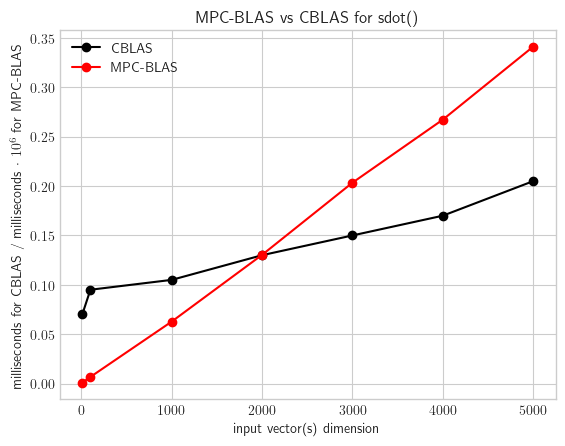
\includegraphics{"./02_postamble/images/mpc-blas-timings-graph.png"}
    \caption[Οι ενδιάμεσες τιμές του χρόνου εκτέλεσης επεξεργαστή (CPU time) της συνάρτησης SDOT για τις βιβλιοθήκες MPC-BLAS και OpenBLAS για συνεχώς μεγαλύτερη είσοδο]{Οι ενδιάμεσες τιμές του χρόνου εκτέλεσης επεξεργαστή (CPU time) της συνάρτησης SDOT για τις βιβλιοθήκες MPC-BLAS και OpenBLAS για συνεχώς μεγαλύτερη είσοδο. Η MPC-BLAS εκτελείται τοπικά σε δύο διαφορετικές διεργασίες, όπου η κάθε διεργασία έτρεχε σε 5 νήματα. Όλες οι τιμές για την MPC-BLAS λήφθηκαν μέσω της εντολής \mintinline{cpp}{# define PRINT_PERFORMANCE_STATS} της βιβλιοθήκης ABY ενώ για την CBLAS μέσω του χρονομέτρου \mintinline{cpp}{std::chrono} της C++.}
    \label{fig:mpc-blas-timings-graph}
\end{figure}

Ας κοιτάξουμε ξανά το παραπάνω αποτέλεσμα από μια πιο πρακτική ματιά. Οι χρονικές πολυπλοκότητες του Σχήματος \ref{fig:mpc-blas-timings-graph} είναι άμεσα συσχετισμένες με το πλήθος των πυλών που χρησιμοποιούνται από αυτές τις δύο βιβλιοθήκες σε επίπεδο υλικού. Αν θεωρήσομε το πρωτόκολλο GMW ως τον "εικονικό" επεξεργαστή της MPC-BLAS πράξης, τότε μπορούμε να ισχυριστούμε πως η εκτέλεση ενός αλγορίθμου σε αυτόν τον "εικονικό" επεξεργαστή δεν επηρεάζει την ασυμπτωτική χρονική πολυπλοκότητα του, παρά μόνο εισάγει μια γραμμική καθυστέρηση που εξαρτάται από το μέγεθος του αλγορίθμου αυτού. Δηλαδή, πως σε επίπεδο πραγματικών πυλών υλικού, εισάγει μια γραμμική στο μέγεθος της εισόδου επιβάρυνση. Ωστόσο, αυτός ο ισχυρισμός δεν είναι ιδιαίτερα ισχυρός καθώς εξαρτάται άμεσα από την πλατφόρμα στην οποία τρέχει αυτός ο εικονικός επεξεργαστής, η οποία συμπεριλαμβάνει το λειτουργικό σύστημα, το υλικό, το δίκτυο και αρκετούς ακόμα άγνωστους παράγοντες. Ο ισχυρισμός αυτός ισχύει μόνο στην περίπτωση που θεωρήσουμε πως η πλατφόρμα στην οποία εκτελείται ο εικονικός επεξεργαστής εισάγει κατά μέσο όρο γραμμική επιβάρυνση στον αριθμό των πυλών που χρησιμοποιεί ένα αυθαίρετο πρόγραμμα.